\documentclass[a4paper]{article}
\usepackage[T1]{fontenc}
\usepackage[utf8x]{inputenc}
\usepackage[english,russian]{babel}
\usepackage{multicol}
\usepackage{fancyhdr}
\usepackage[warn]{mathtext}
\usepackage{graphicx}
\usepackage{microtype}
\usepackage{wrapfig}
\usepackage{amsmath}
\usepackage{floatflt}
\usepackage{geometry} \geometry{verbose,a4paper,tmargin=2cm,bmargin=2cm,lmargin=1.5cm,rmargin=1.5cm}
\usepackage{float}
\usepackage{amssymb}
\usepackage{caption}
\usepackage{epsfig}
\usepackage{newunicodechar}

\begin{document}
\newcommand{\apple}{\char"F8FF}

\begin{titlepage}
	\centering
	\vspace{5cm}
    {\scshape\LARGE Московский физико-технический институт\par}
    
\begin{figure}[H]
\begin{center}

\includegraphics[scale = 0.4]{mipt_rus_text.png}
\label{default}
\end{center}
\end{figure}

	\vspace{3cm}
	{\scshape\Large Лабораторная работа по общей физике \par}
	\vspace{1cm}
    {\huge\bfseries  4.2 Исследование энергетического спектра $\beta$-частиц и определение их 
    максимальной энергии при помощи магнитного спектрометра \par}
	\vspace{1cm}
	\vfill
\begin{flushright}
	{\large выполнил студент Б04-852 группы ФЭФМ}\par
	\vspace{0.3cm}
	{\LARGE Яромир Водзяновский}
\end{flushright}
	
	\vfill
Долгопрудный, 2020
% Bottom of the page
\end{titlepage}

\pagestyle{fancy} 
\fancyhead[L]{Спектр $\beta$-частиц         $\sim  \hat(\, ^{\circ}  \omega  ^{\circ} \, \hat) \sim$}
\fancyhead[R]{Квантовая физика}
\fancyhead[C]{}
\fancyfoot[C]{ \noindent\rule{\textwidth}{0.4pt} \thepage }

\tableofcontents

\newpage


\section{Цель работы}

С помощью магнитного спектрометра исследовать энергетический спектр $\beta$-частиц при распаде
ядер $^{137}Cs$ и определение их максимальной энергии.Калибровка спектрометра осуществляется
по энергии электронов внутренней конверсии $^{137}Cs$.

\section{Оборудование}
\begin{enumerate}
    \item Магнитный спектрометр с "короткой линзой"
    \item Высоковольтный и низковольтный выпрямители
    \item Форвакуумный насос и вакууметр
    \item ЭВМ
\end{enumerate}


\section{Теория}

\textbf{$\beta$-распадом} называется самопроизвольное превращение ядер, при котором их массовое
число не меняется, а заряд увеличивается или уменьшается на единицу. В нашем случае имеем дело 
с электронным распадом:
$${_Z^A}X \rightarrow {_{Z+1}^A}X + e^- + \tilde{\nu}$$

Освобождающаяся энергия делится между электроном и антинейтрино, дочернему ядру достается очень
мало.

Вид спектра $\beta$-частиц показан на рис.\ref{p1}. $W(p_e)$ есть плотность вероятности. А 
$W(p_e)dp_e$ есть вероятность того, что $\beta$-частица получит импульс в интервале $(p_e, \; p_e+dp_e)$.

\begin{wrapfigure}[17]{l}{145pt}
    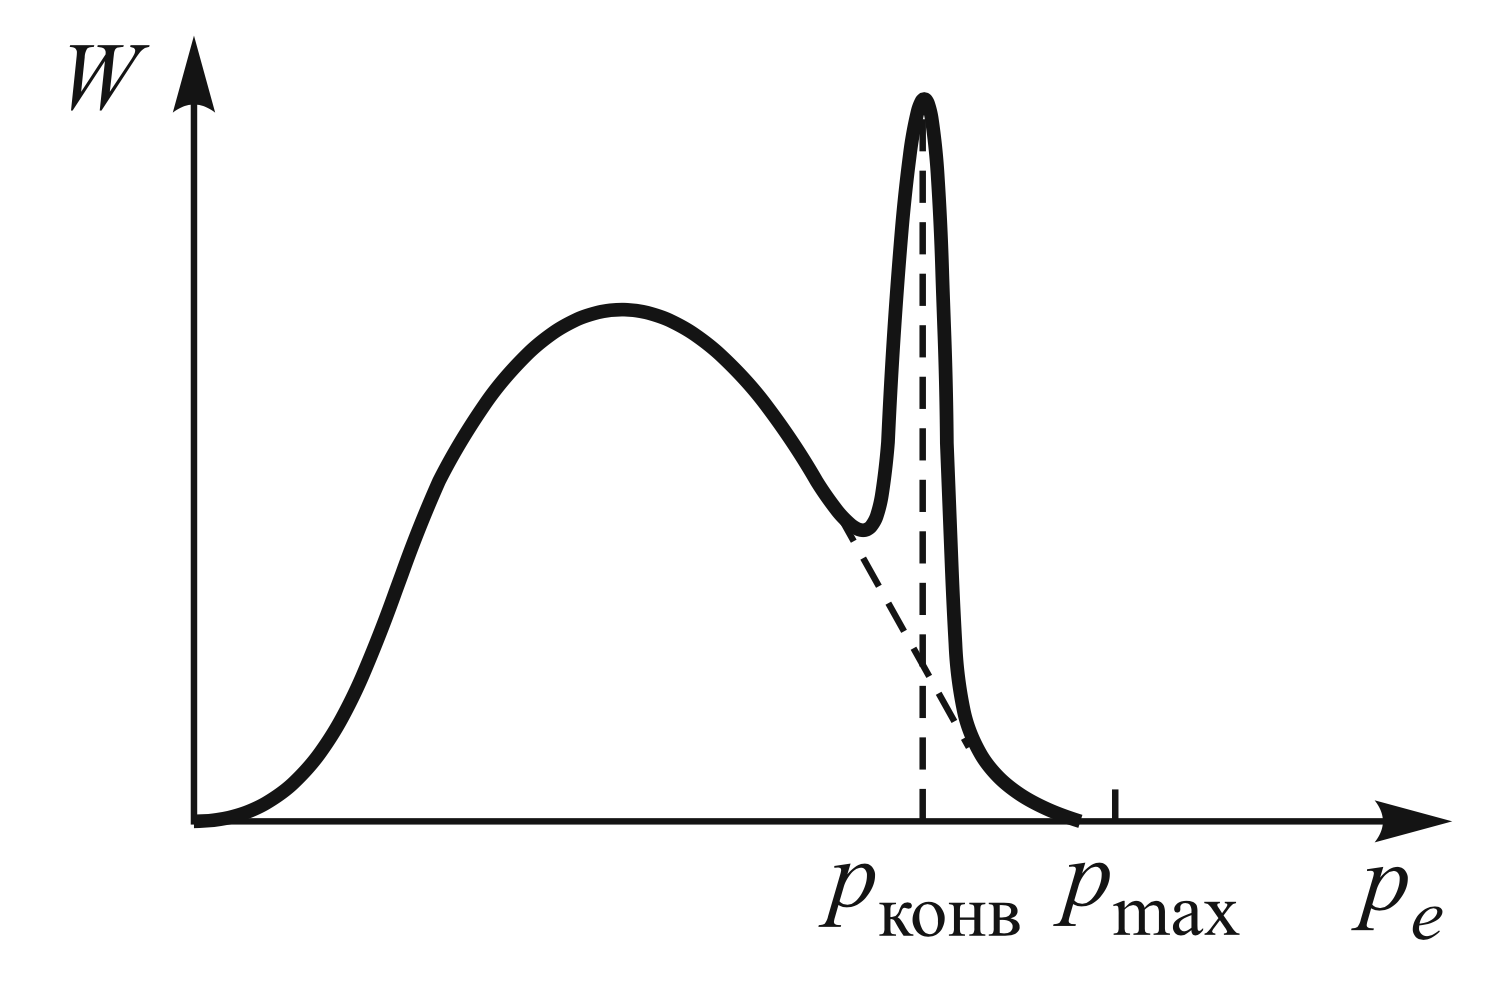
\includegraphics[scale = 0.2]{p1.png}
    \caption{Форма спектра $\beta$-частиц при разрешенных переходах}
    \label{p1}
\end{wrapfigure}

Вероятность $\beta$-распада пропорциональна фазовому объему в векторном пространстве имупульсов
электронов и антинейтрино. Интервалу $(p_e, \; p_e+dp_e)$ соответсввет шаровой слой объема 
$4\pi p_e^2 dp_e$. В пространстве импульсов, уносимых антинейтрино, выделятеся шаровой слой 
площадью $4 \pi p_{\nu}^2$, значит:

\begin{equation}
    W(p_e) dp_e \propto p_e^2 p_{\nu}^2 dp_e 
    \label{eq1}
\end{equation}

Выразим в этом соотношении $p_{\nu}$ через $p_e$. Масса антинейтрино равна нулю, значит:

\begin{equation}
    p_{\nu} = E_{\nu} / c = (T_{max} - T_e)/c
    \label{eq2}
\end{equation}

$E_{\nu}$ - кинетическая энергия антинейтрино, $T_{max}$ - масимально возможная кнетическая энергия
электрона. $T_e$ - фактическая энергия электрона. Подставляя \ref{eq2} в \ref{eq1} получим:

\begin{equation}
    W(p_e)dp_e \propto p_e^2 (T_{max} - T_e)^2 dp_e
    \label{eq3}
\end{equation}

Кинетическая энергия электрона и его импульс связаны следующим:

\begin{equation}
    T_e = \sqrt{p_e^2 c^2 + m_e^2 c^4} - m_e c^2
    \label{eq4}
\end{equation}

Следует:

\begin{equation}
    T_{max} - T_e = c (\sqrt{p_{max}^2 + m_e^2 c^2} - \sqrt{p_e^2 + m_e^2 c^2})
    \label{eq5}
\end{equation}

Уравнение (\ref{eq5}) описывает спектр как широкий колокол (рис.\ref{p1}) 

Дочерние ядра нередко бывают возбужденными, поэтому они могут излучать $\gamma$-квант или 
передавать избыток электрону на внутренней оболочке. Такие излучаемые электроны называются 
\textbf{конверсионными}. На спектре  (рис.\ref{p1}) видна монохроматическая линия, ширина
которой обусловлена лишь разрешающей способностью спектрометра.

\section{Экспериментальная установка}

Энергию частиц определяют с помощью $\beta$-спектрометра. В работе используется 
магнитный спеткрометр с "короткой линзой", сцинтиллятором и ФЭУ. По расчету, 
тонкая катушка эквивалент на линзе:

\begin{equation}
    \frac{1}{f} \approx \frac{I^2}{p_e^2}
    \label{eq6}
\end{equation}

\begin{figure}[h]
	\begin{center}
	\begin{minipage}[h]{0.45\linewidth}
	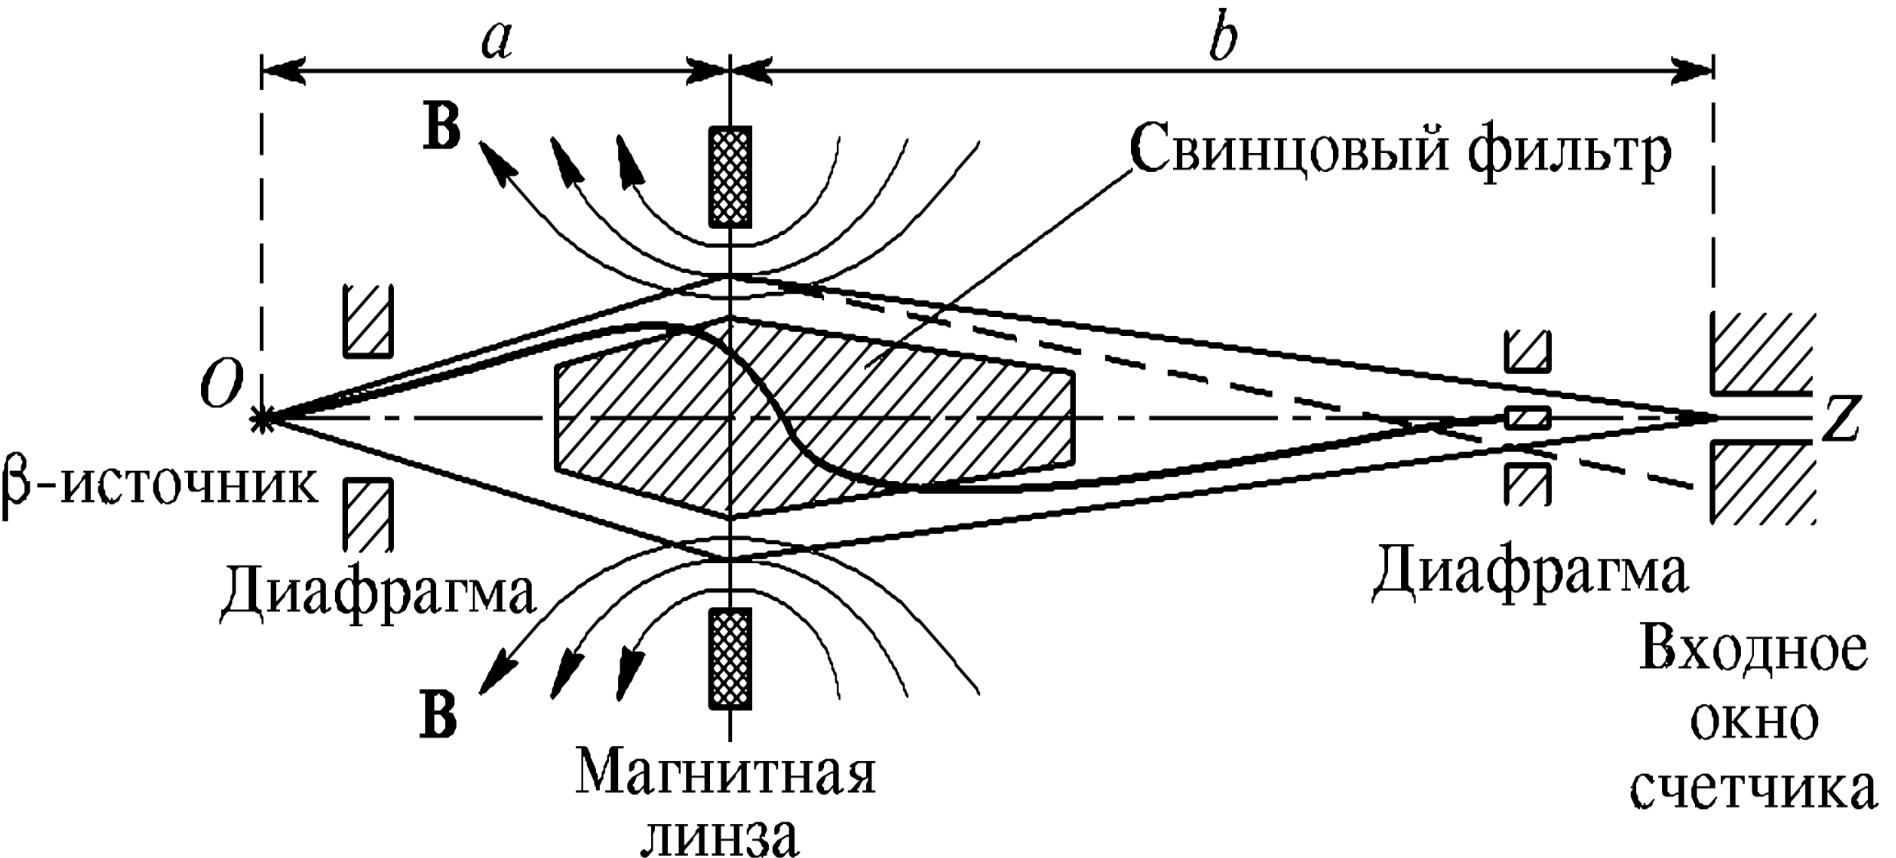
\includegraphics[width=1\linewidth]{p2.png}
	\caption{Схема $\beta$-спектрометра с короткой магнитной линзой} 
	\label{p2}
	\end{minipage}
	\hfill 
	\begin{minipage}[h]{0.45\linewidth}
	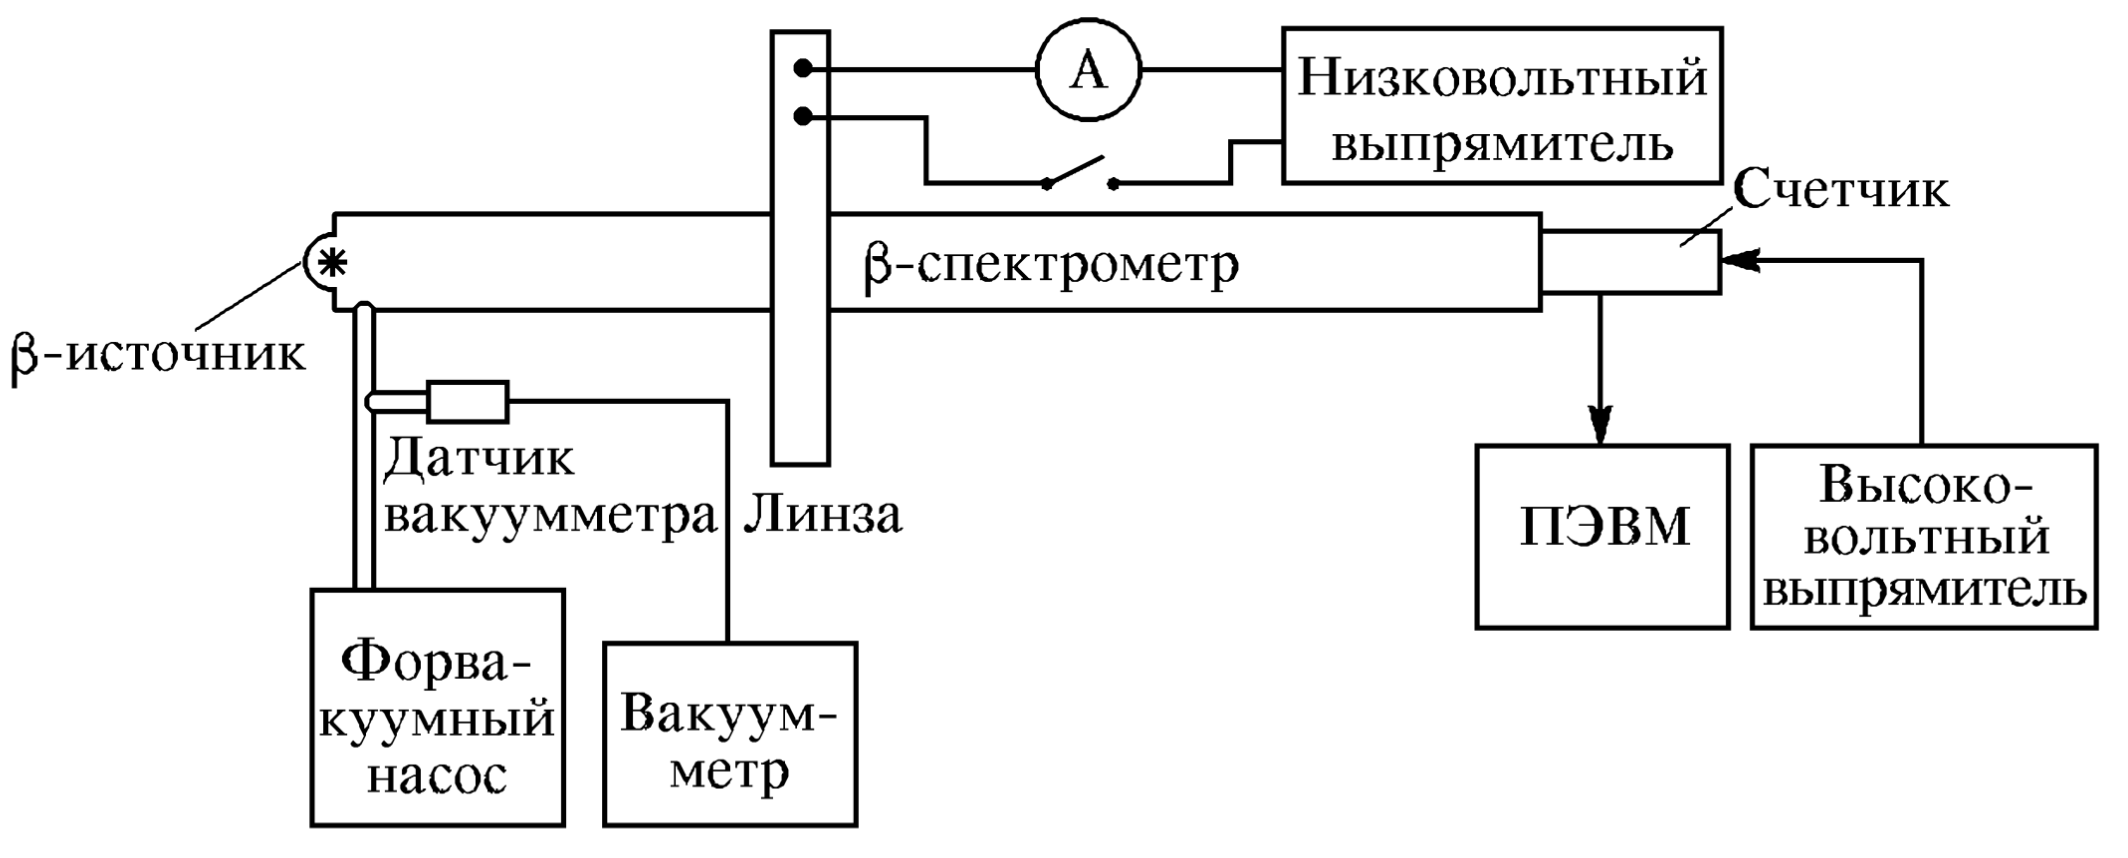
\includegraphics[width=1\linewidth]{p3.png}
	\caption{Блок-схема измерительного комлпекса}
	\label{p3}
	\end{minipage}
	\end{center}
\end{figure}

При заданной силе тоув на входное окно счетчика фокусируются электоны с 
определенным значением импульса. Импульс сфокусированнх электонов пропорционален 
величине тока I:

\begin{equation}
    p_e = k\cdot I
    \label{eq7}
\end{equation}

Константа прибора k определяется по известной конверсионной линии.

Линза обладает абберацией, поэтому установлены кольцевые диафрагмы, ограничивающие
углы вылетов электронов. Также установлен свинцовый фильтр, сдерживающий $\gamma$-кванты 
и электроны, летящие прямо. Величина $\Delta p_e$ - разрешающая способность.

Рассмотрим связь между числом частиц, регистрируемых установкой, и функцией $W(p_e)$, 
определяемой формулой (\ref{eq3}):

\begin{equation}
    N(p_e) \approx W(p_e) \Delta p_e 
    \label{eq8}
\end{equation}

Фокус линзы зависит от импульса, частицы проходят мимо при больших $\Delta f$, 
продиффиренцируем (\ref{eq6})

\begin{equation}
    \Delta p_e = \frac{1}{2} \frac{\Delta f}{f} p_e
    \label{eq9}
\end{equation}

Таким образом, ширина интервала $\Delta p_e$ пропорциональна импульсу. Подставим 
(\ref{eq9}) в (\ref{eq8}):

\begin{equation}
    N(p_e) = C \cdot W(p_e) p_e
    \label{eq10}
\end{equation}

где С - некоторая константа.

Давление в спектрометре поддерживается на уровне 0.1 Торр и измеряется вакууметром.
Откачка освществляется форвакуумным насосом. Высокое напряжение на ФЭУ подается
от стабилизированного выпрямителя.


\section{Ход работы}

\begin{enumerate}
    \item Включаем пересчетный прибор, высоковольтный выпрямитель и вакууметр. Откачиваем давление
    до 0.1 Торр форвакуумным насосом.
    \item Включаем рабочее напряжение на ФЭУ
    \item Убеждаемся, что спектрометр корректно работает, для этого меняем ток в катушке от 1 до 
    4 А, мы должны наблюдать силный рост счетов с повышением тока.
    \item Проведем измерения, увеличивая силу тока на 0.2 А в интервале от 0 до 5 А.
    \item Выключим ток в линзе и измерим фоновый счет спектрометра $\sim 0.8 \pm 2\%$
    \item Занесем данные в таблицу \ref{t1}.
    \begin{table}[H]
        \centering
        \caption{}
        \label{t1}
        \begin{tabular}{|c|c|c|c|c|c|c|}
            \hline
            I, A & N & N-Nф & Nф & p, кэВ/с & T, кэВ & mkFermi \\
            \hline \hline
            0 & 0.75 & -0.05 & 0.8 & 0 & 0 & 0 \\ \hline
            0.2 & 0.737 & -0.063 & 0.8 & 48.2 & 2.3 & 0 \\ \hline
            0.4 & 0.712 & -0.088 & 0.8 & 96.4 & 9 & 0 \\ \hline
            0.6 & 0.825 & 0.025 & 0.8 & 144.5 & 20 & 90.417 \\ \hline
            0.8 & 0.987 & 0.187 & 0.8 & 192.7 & 35.1 & 161.7047 \\ \hline
            1 & 1.437 & 0.637 & 0.8 & 240.9 & 53.9 & 213.4799 \\ \hline
            1.2 & 1.424 & 0.624 & 0.8 & 289.1 & 76.1 & 160.7966 \\ \hline
            1.4 & 2.437 & 1.637 & 0.8 & 337.2 & 101.2 & 206.5732 \\ \hline
            1.6 & 2.549 & 1.749 & 0.8 & 385.4 & 129 & 174.7902 \\ \hline
            1.8 & 2.949 & 2.149 & 0.8 & 433.6 & 159.2 & 162.3662 \\ \hline
            2 & 3.249 & 2.449 & 0.8 & 481.8 & 191.3 & 147.9894 \\ \hline
            2.2 & 3.536 & 2.736 & 0.8 & 529.9 & 225.2 & 135.5923 \\ \hline
            2.4 & 3.386 & 2.586 & 0.8 & 578.1 & 260.6 & 115.6948 \\ \hline
            2.6 & 3.261 & 2.461 & 0.8 & 626.3 & 297.3 & 100.0961 \\ \hline
            2.8 & 2.861 & 2.061 & 0.8 & 674.5 & 335.2 & 81.9679 \\ \hline
            3 & 2.736 & 1.936 & 0.8 & 722.6 & 374.1 & 71.6349 \\ \hline
            3.2 & 2.037 & 1.237 & 0.8 & 770.8 & 413.8 & 51.9648 \\ \hline
            3.4 & 1.399 & 0.599 & 0.8 & 819.0 & 454.3 & 33.0340 \\ \hline
            3.6 & 1.212 & 0.412 & 0.8 & 867.2 & 495.5 & 25.1369 \\\hline
            3.8 & 1.349 & 0.549 & 0.8 & 915.3 & 537.3 & 26.7670 \\\hline
            4 & 2.649 & 1.849 & 0.8 & 963.5 & 579.6 & 45.4653 \\\hline
            4.2 & 3.661 & 2.861 & 0.8 & 1011.7 & 622.4 & 52.5644 \\\hline
            4.4 & 1.824 & 1.024 & 0.8 & 1059.9 & 665.6 & 29.3315 \\\hline
            4.6 & 0.525 & -0.275 & 0.8 & 1108.0 & 709.2 & 0 \\\hline
            4.8 & 0.337 & -0.463 & 0.8 & 1156.2 & 753.1 & 0 \\\hline
            5 & 0.487 & -0.313 & 0.8 & 1204.4 & 797.3 & 0 \\\hline
        \end{tabular}
    \end{table}
\end{enumerate}


\section{Обработка результатов}

\begin{enumerate}
    \item Вычтем из результатов измеренный фон и построим график остчетов от тока в катушке.
    \begin{figure}[H]
        \begin{center}
        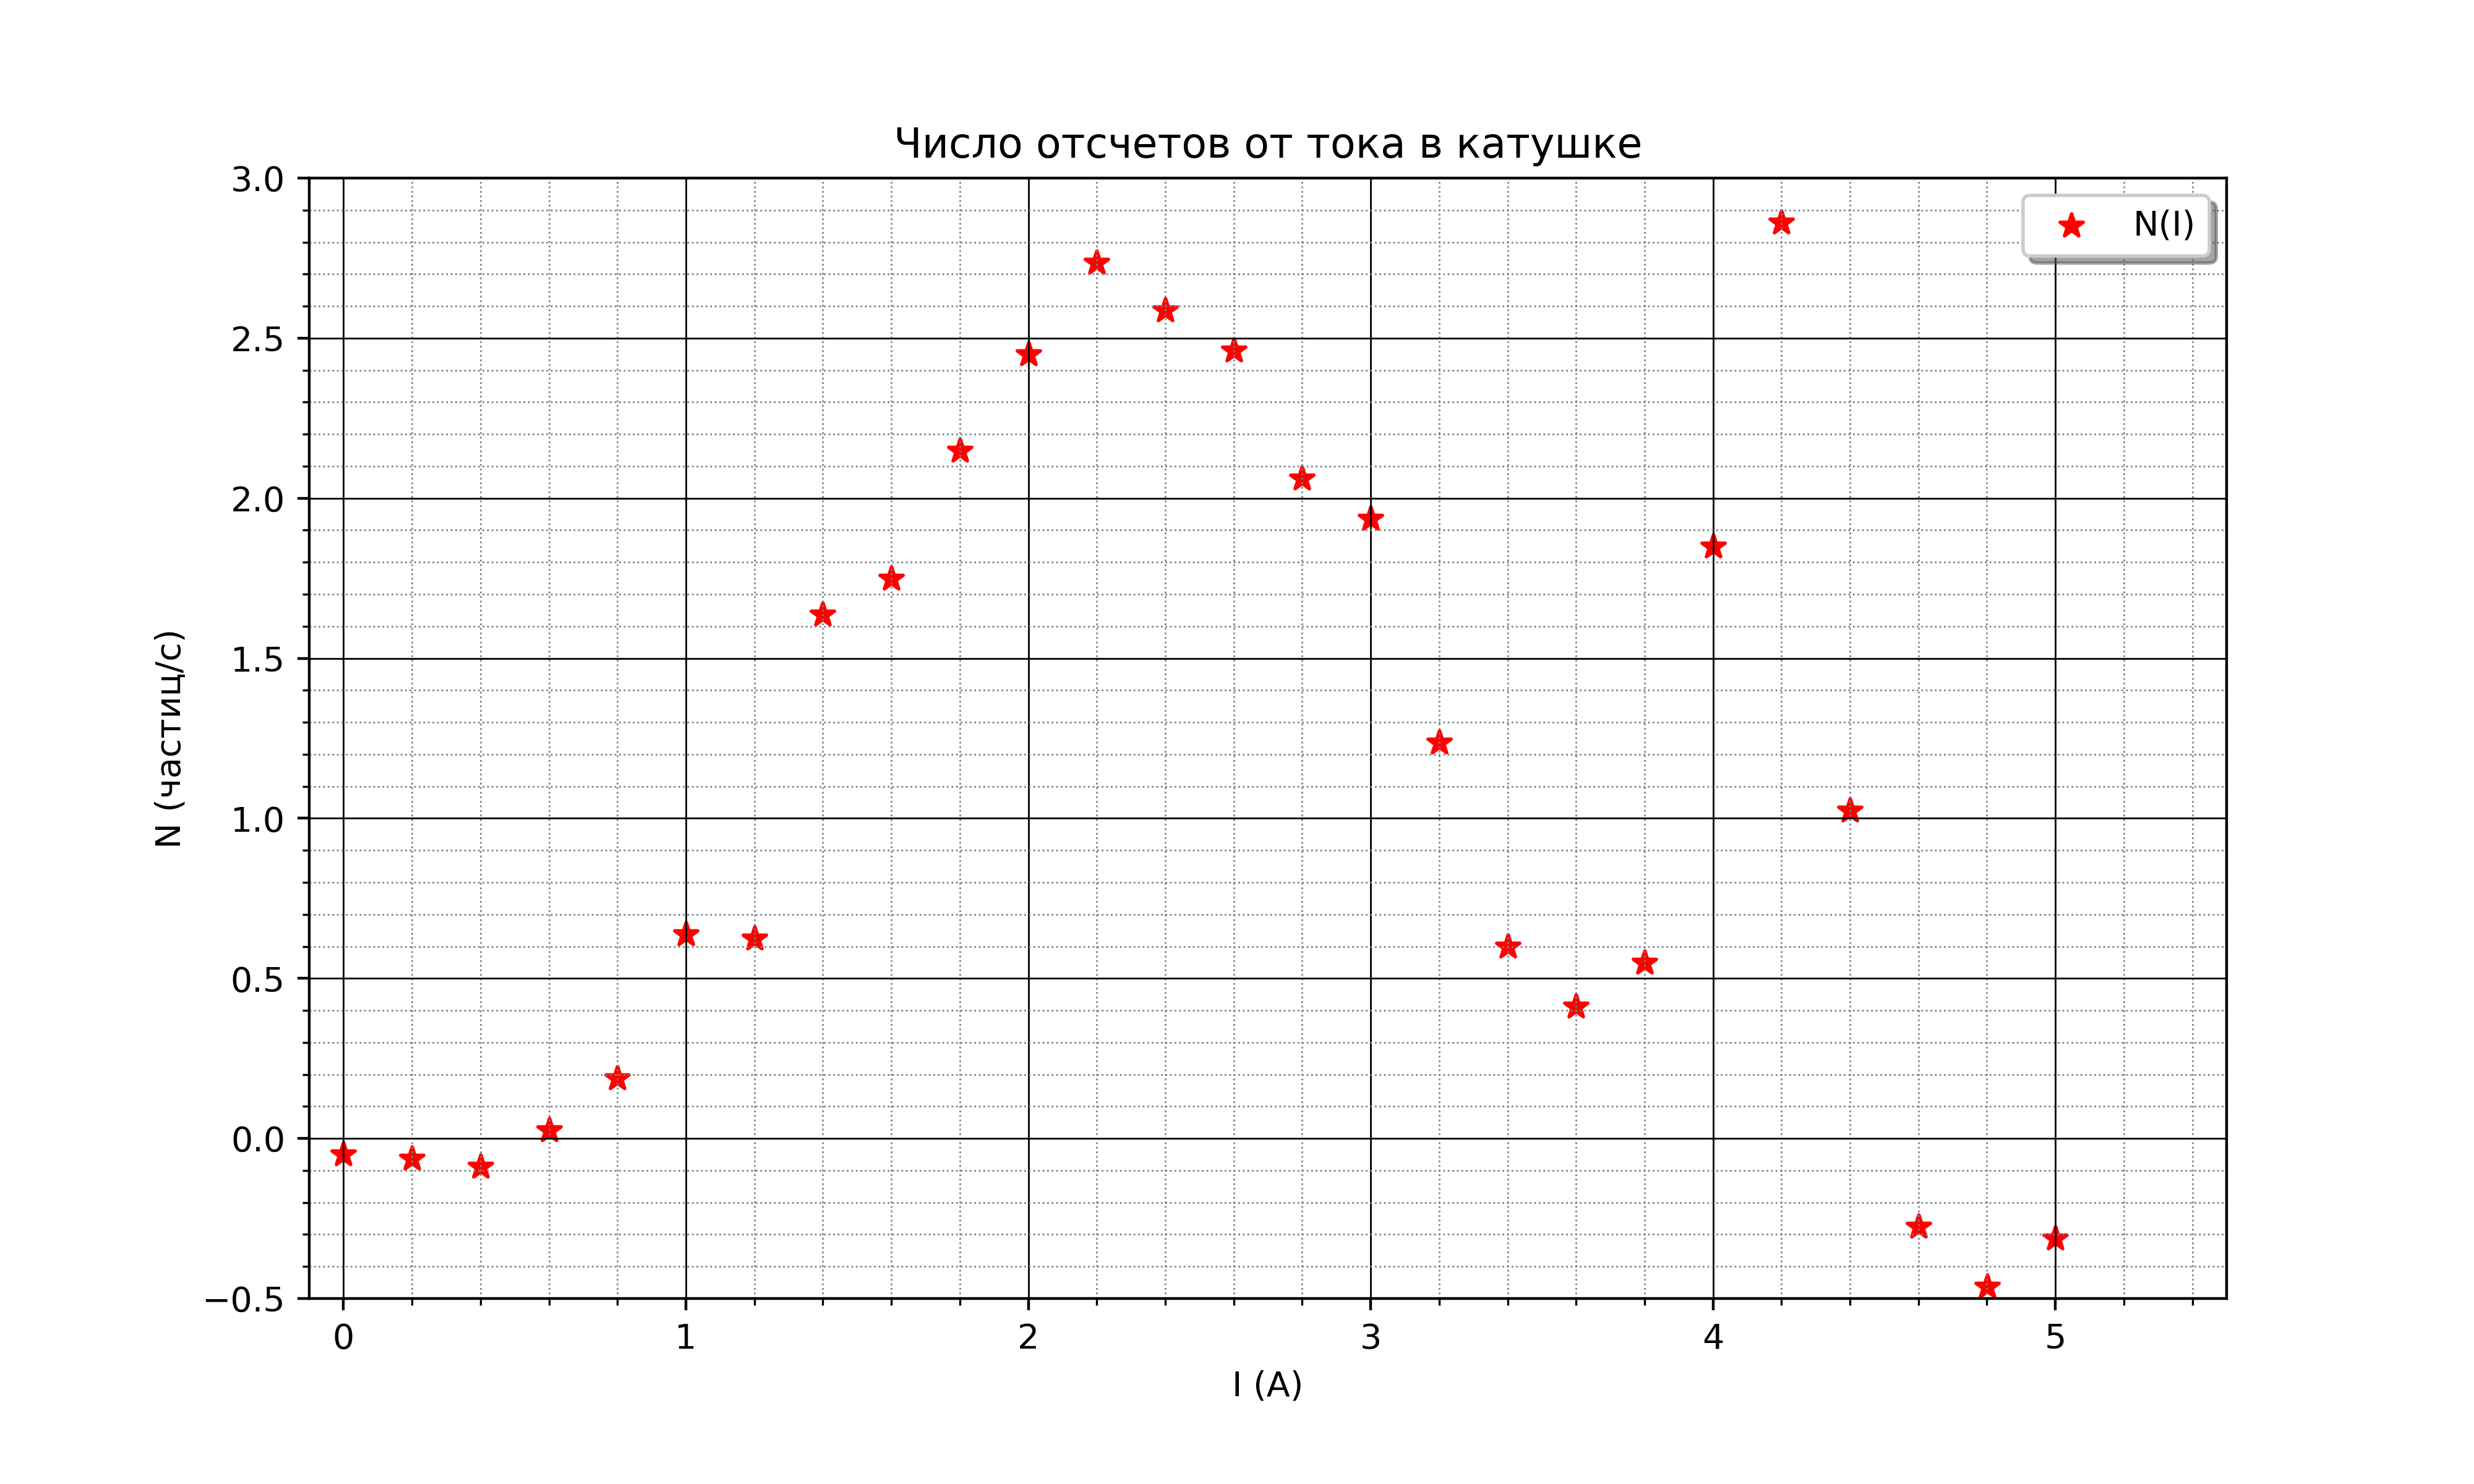
\includegraphics[scale = 0.54]{N(I).png}
        \caption{}
        \label{g1}
        \end{center}
    \end{figure}

    По значению $T_{\text{конв}} = 0.624$МэВ по формуле (\ref{eq7}) определим константу прибора
    $k \approx 240.9$

    Построим графики N(T) и $N(p_e)$

    \begin{figure}[h]
        \begin{center}
        \begin{minipage}[h]{0.47\linewidth}
        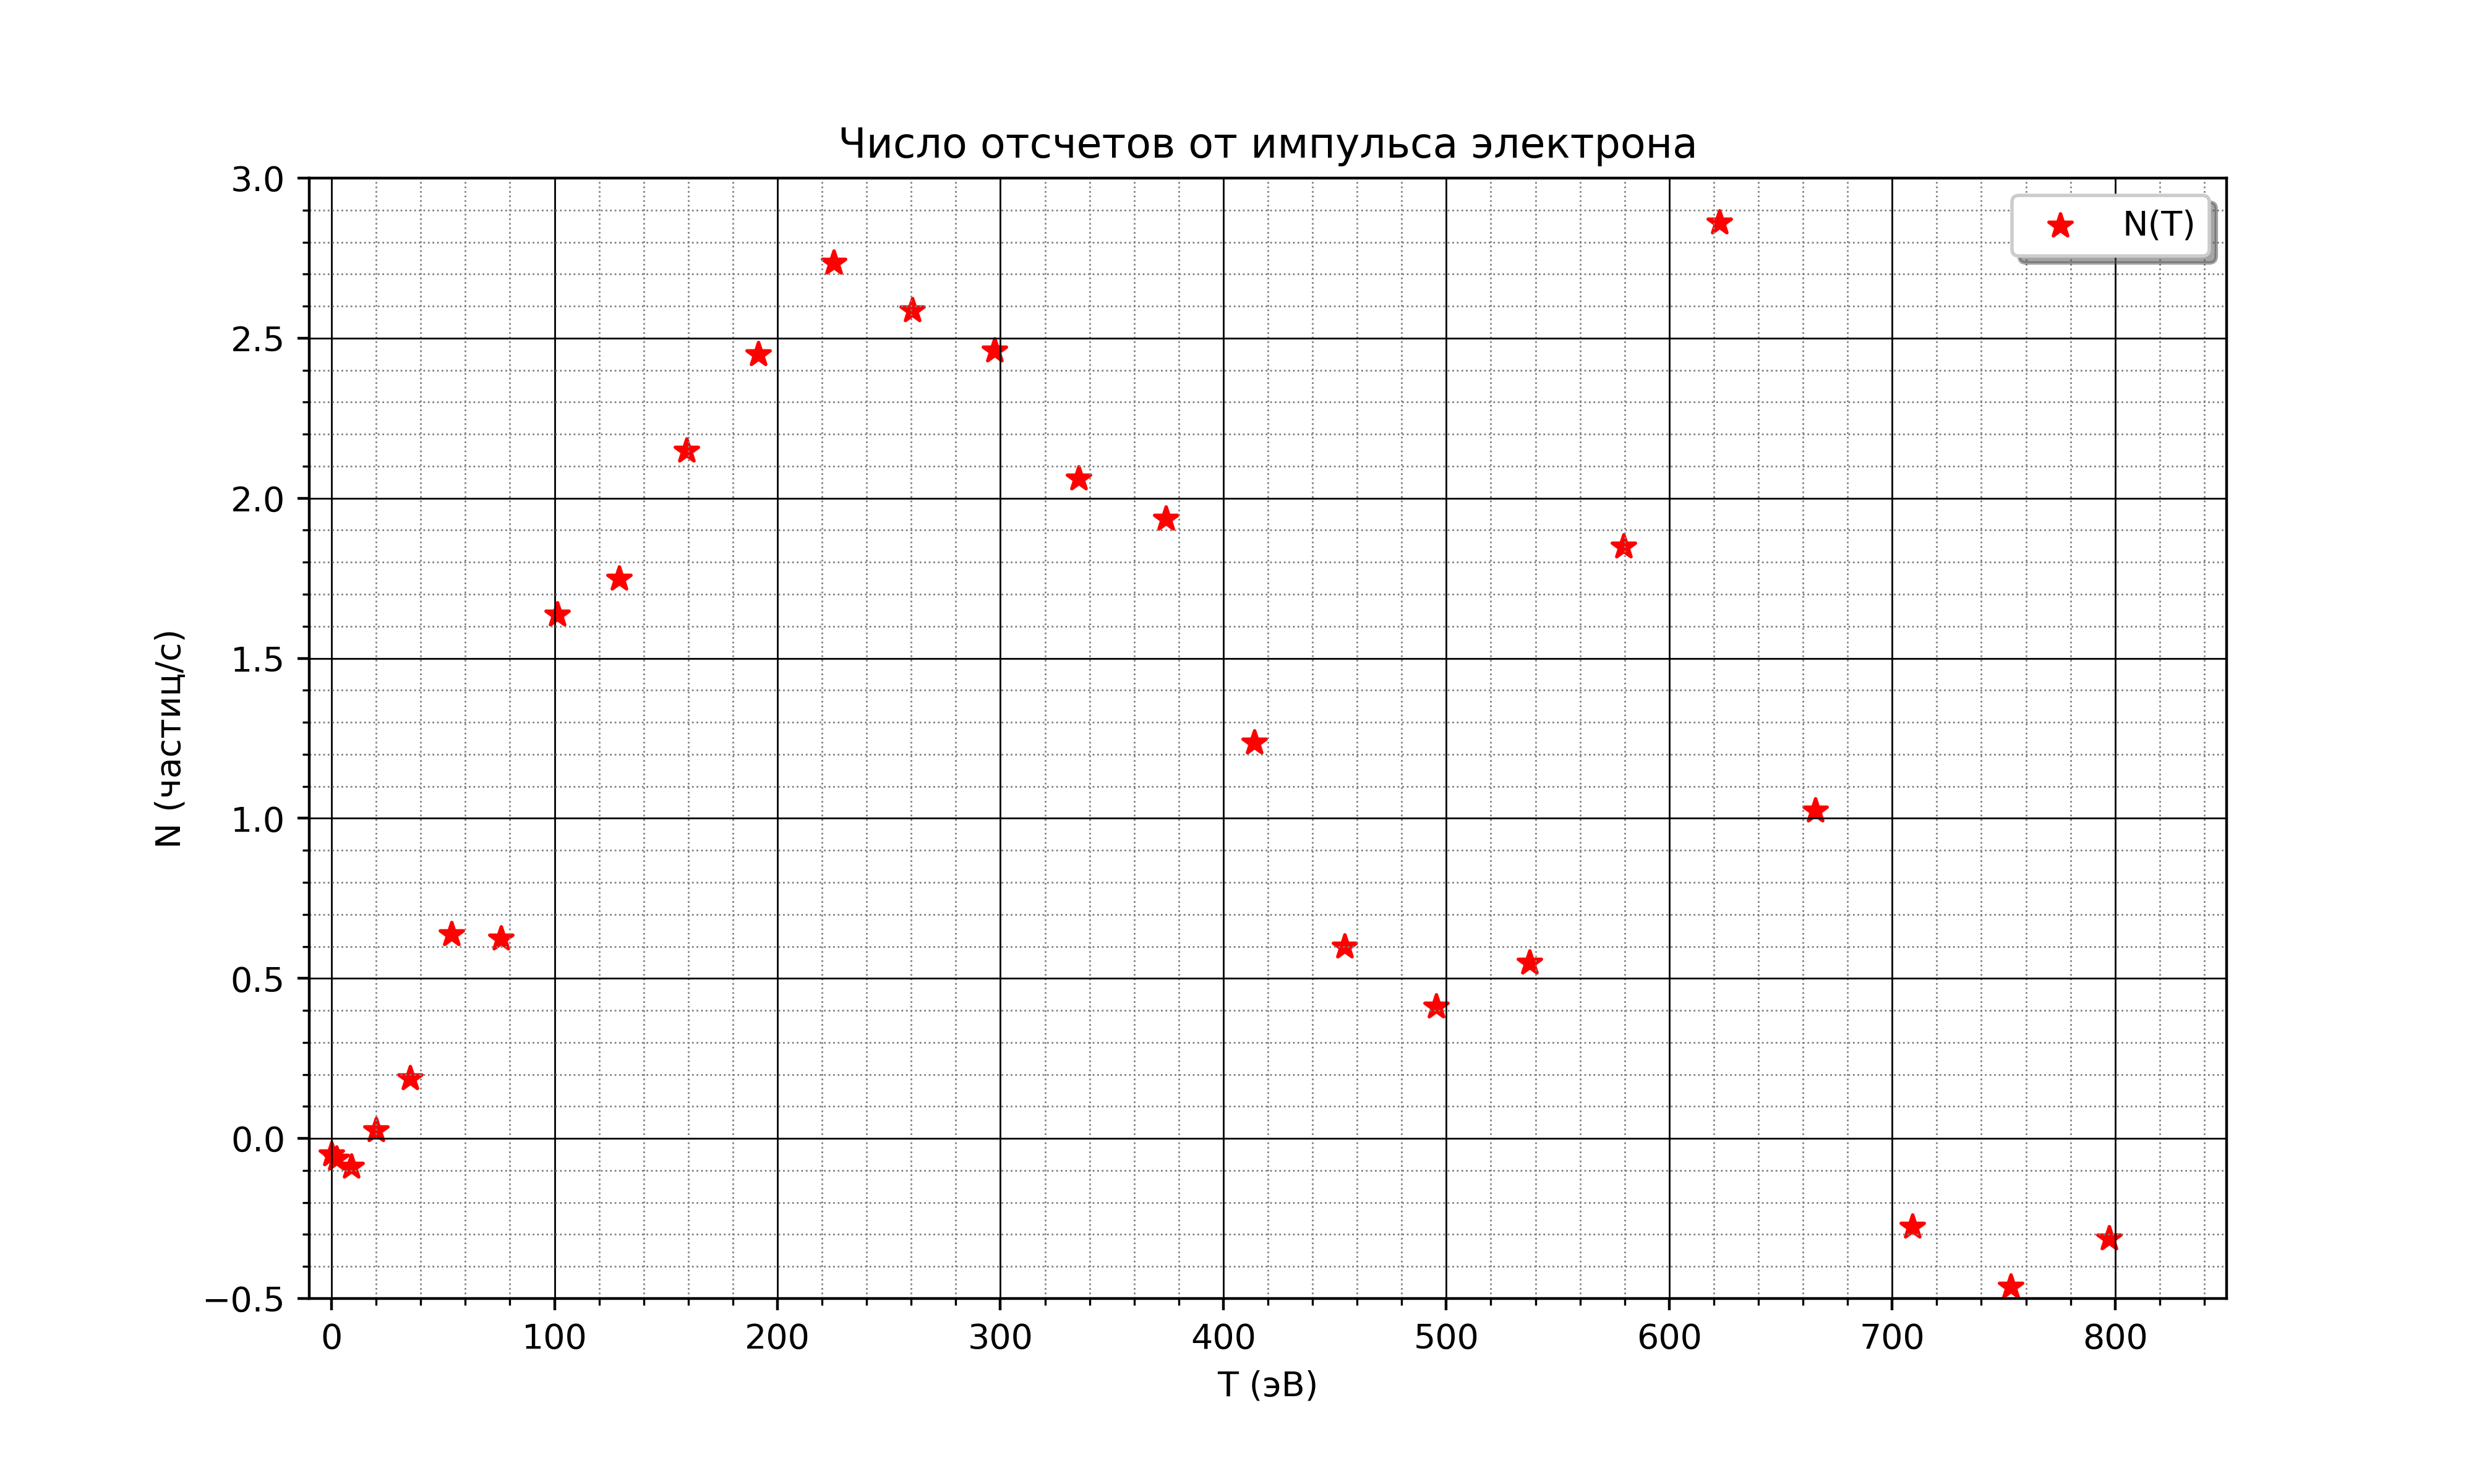
\includegraphics[width=1\linewidth]{N(T).png}
        \caption{} 
        \label{N(T)}
        \end{minipage}
        \hfill 
        \begin{minipage}[h]{0.47\linewidth}
        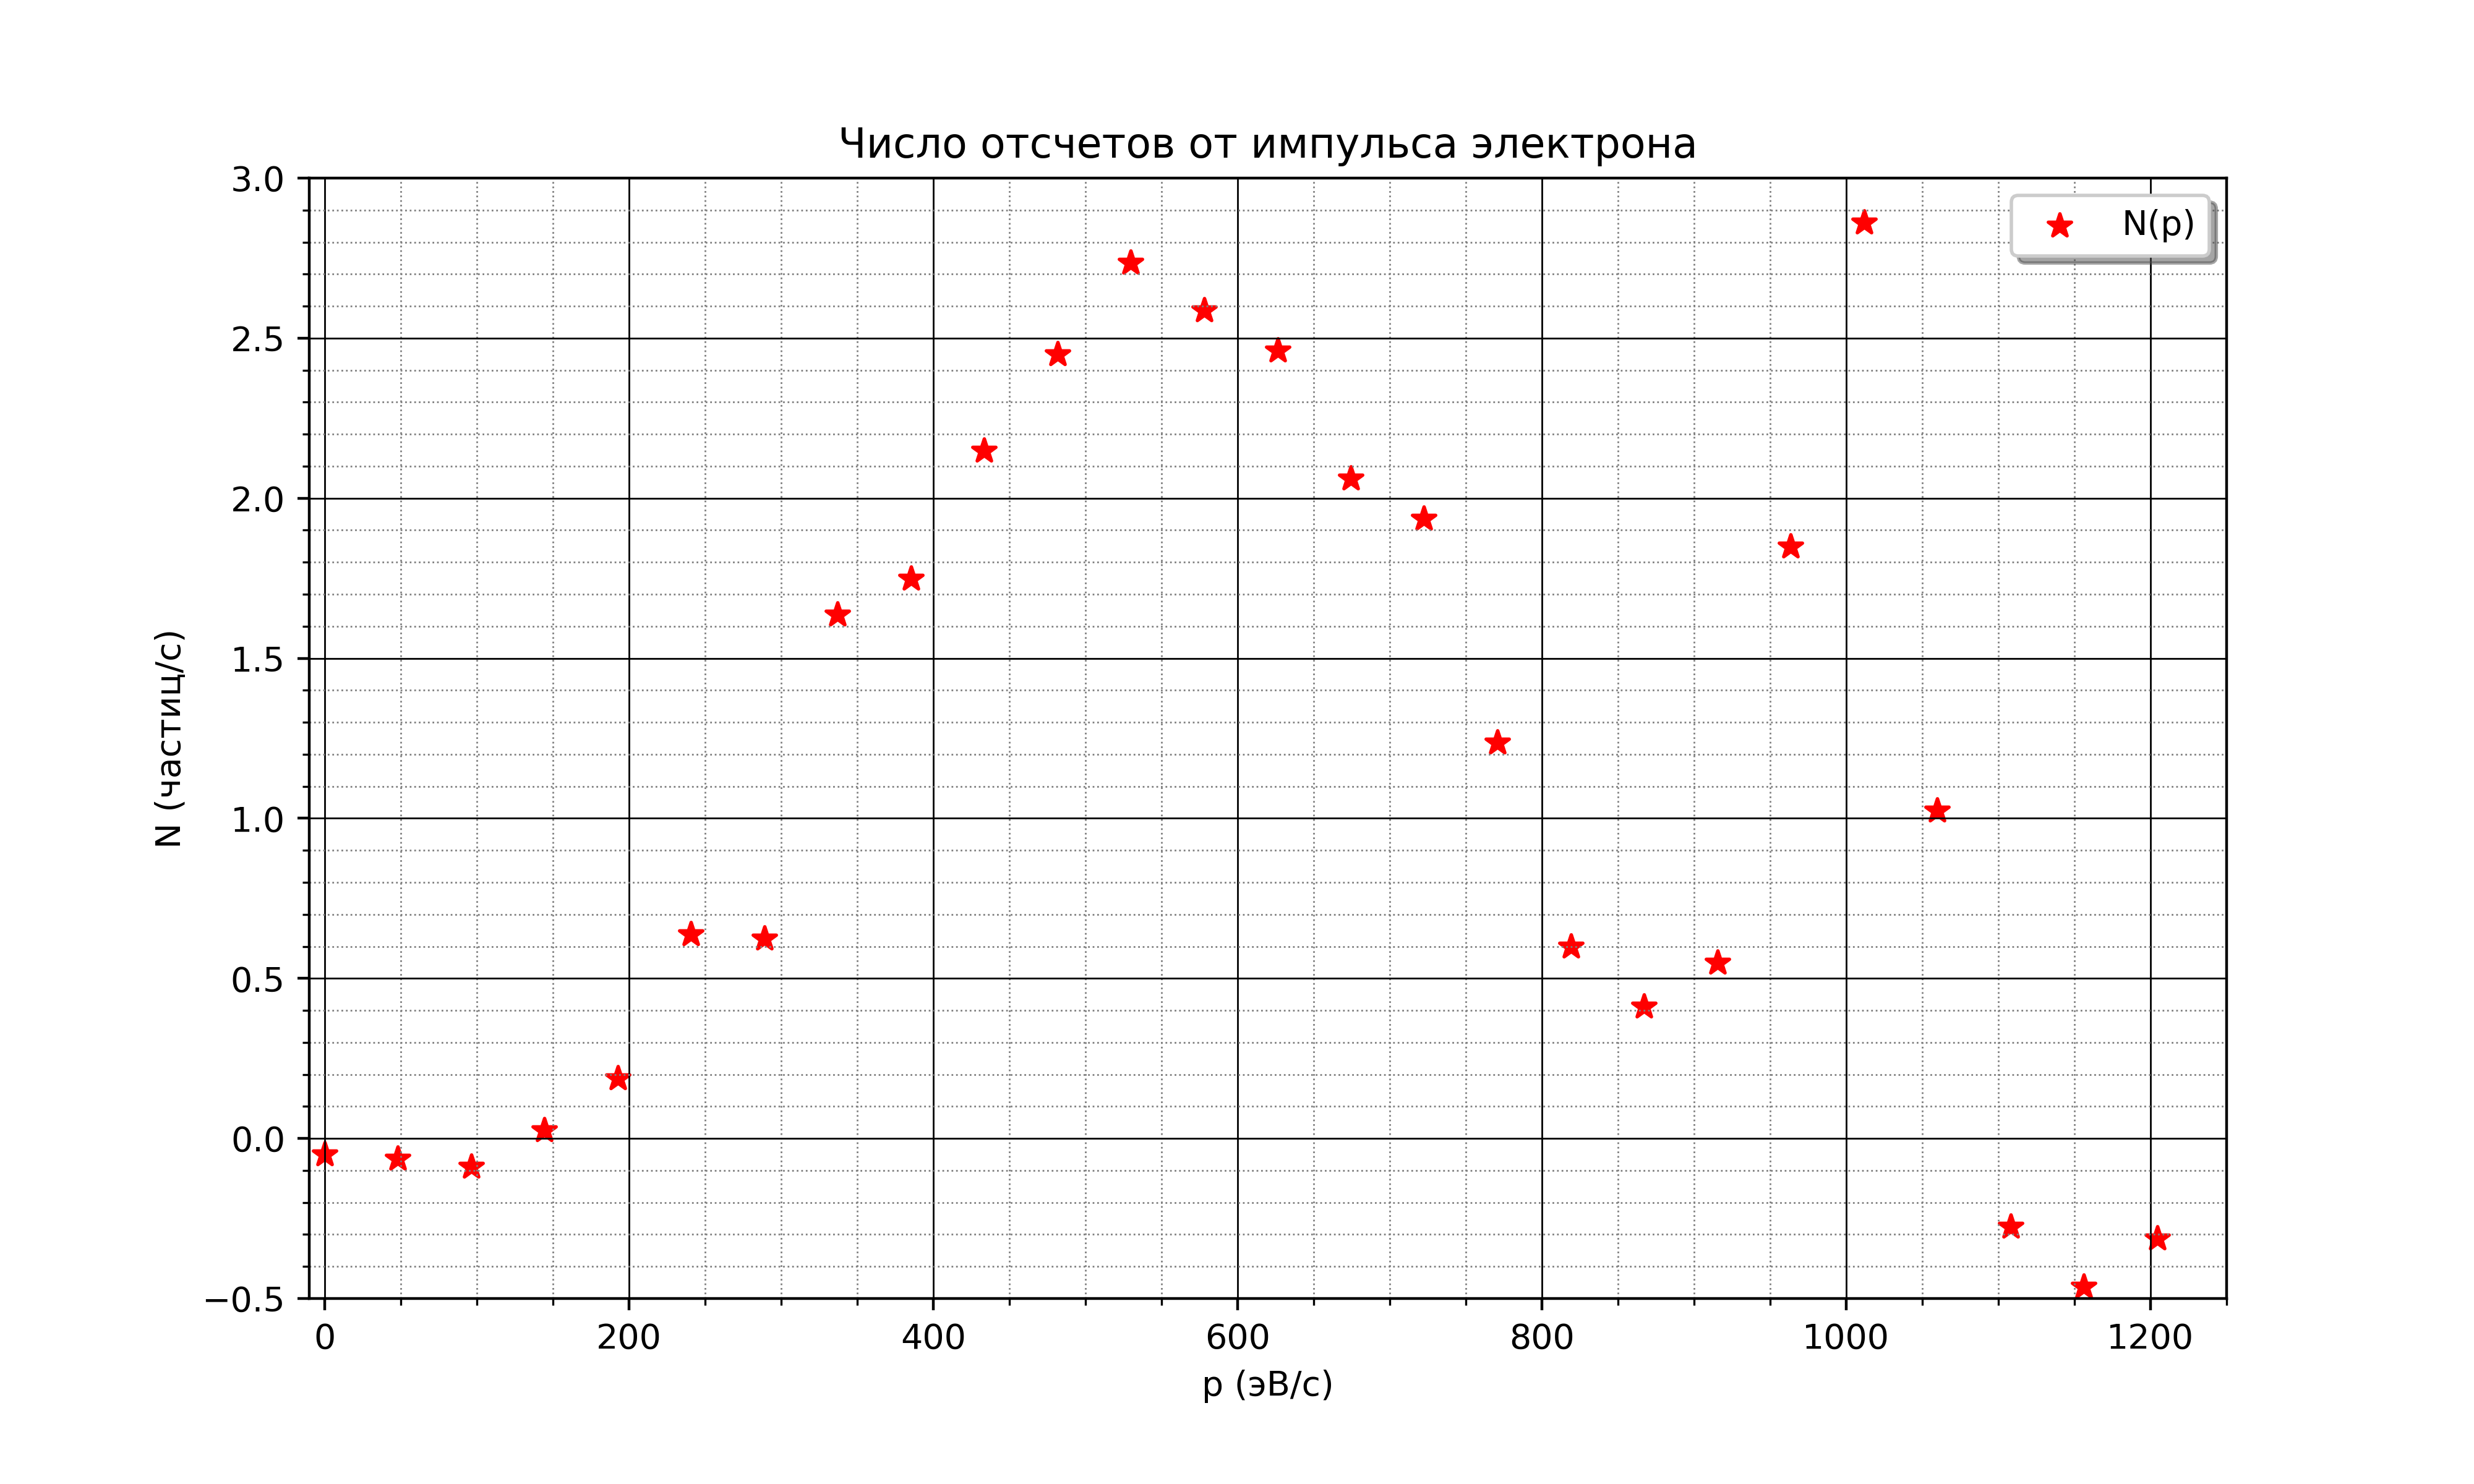
\includegraphics[width=1\linewidth]{N(p).png}
        \caption{}
        \label{N(p)}
        \end{minipage}
        \end{center}
    \end{figure}

    \item Определим $T_{max}$ с помощью графика Ферми. Подставим в (\ref{eq3}) значение $W(p_e)$
    из (\ref{eq10}) и разделим на $\Delta p_e$:

    \begin{equation}
        \sqrt{N(p_e)}\; / \; p^{3/2} \propto T_{max} - T
        \label{eq11}
    \end{equation}

    \begin{figure}[H]
        \begin{center}
        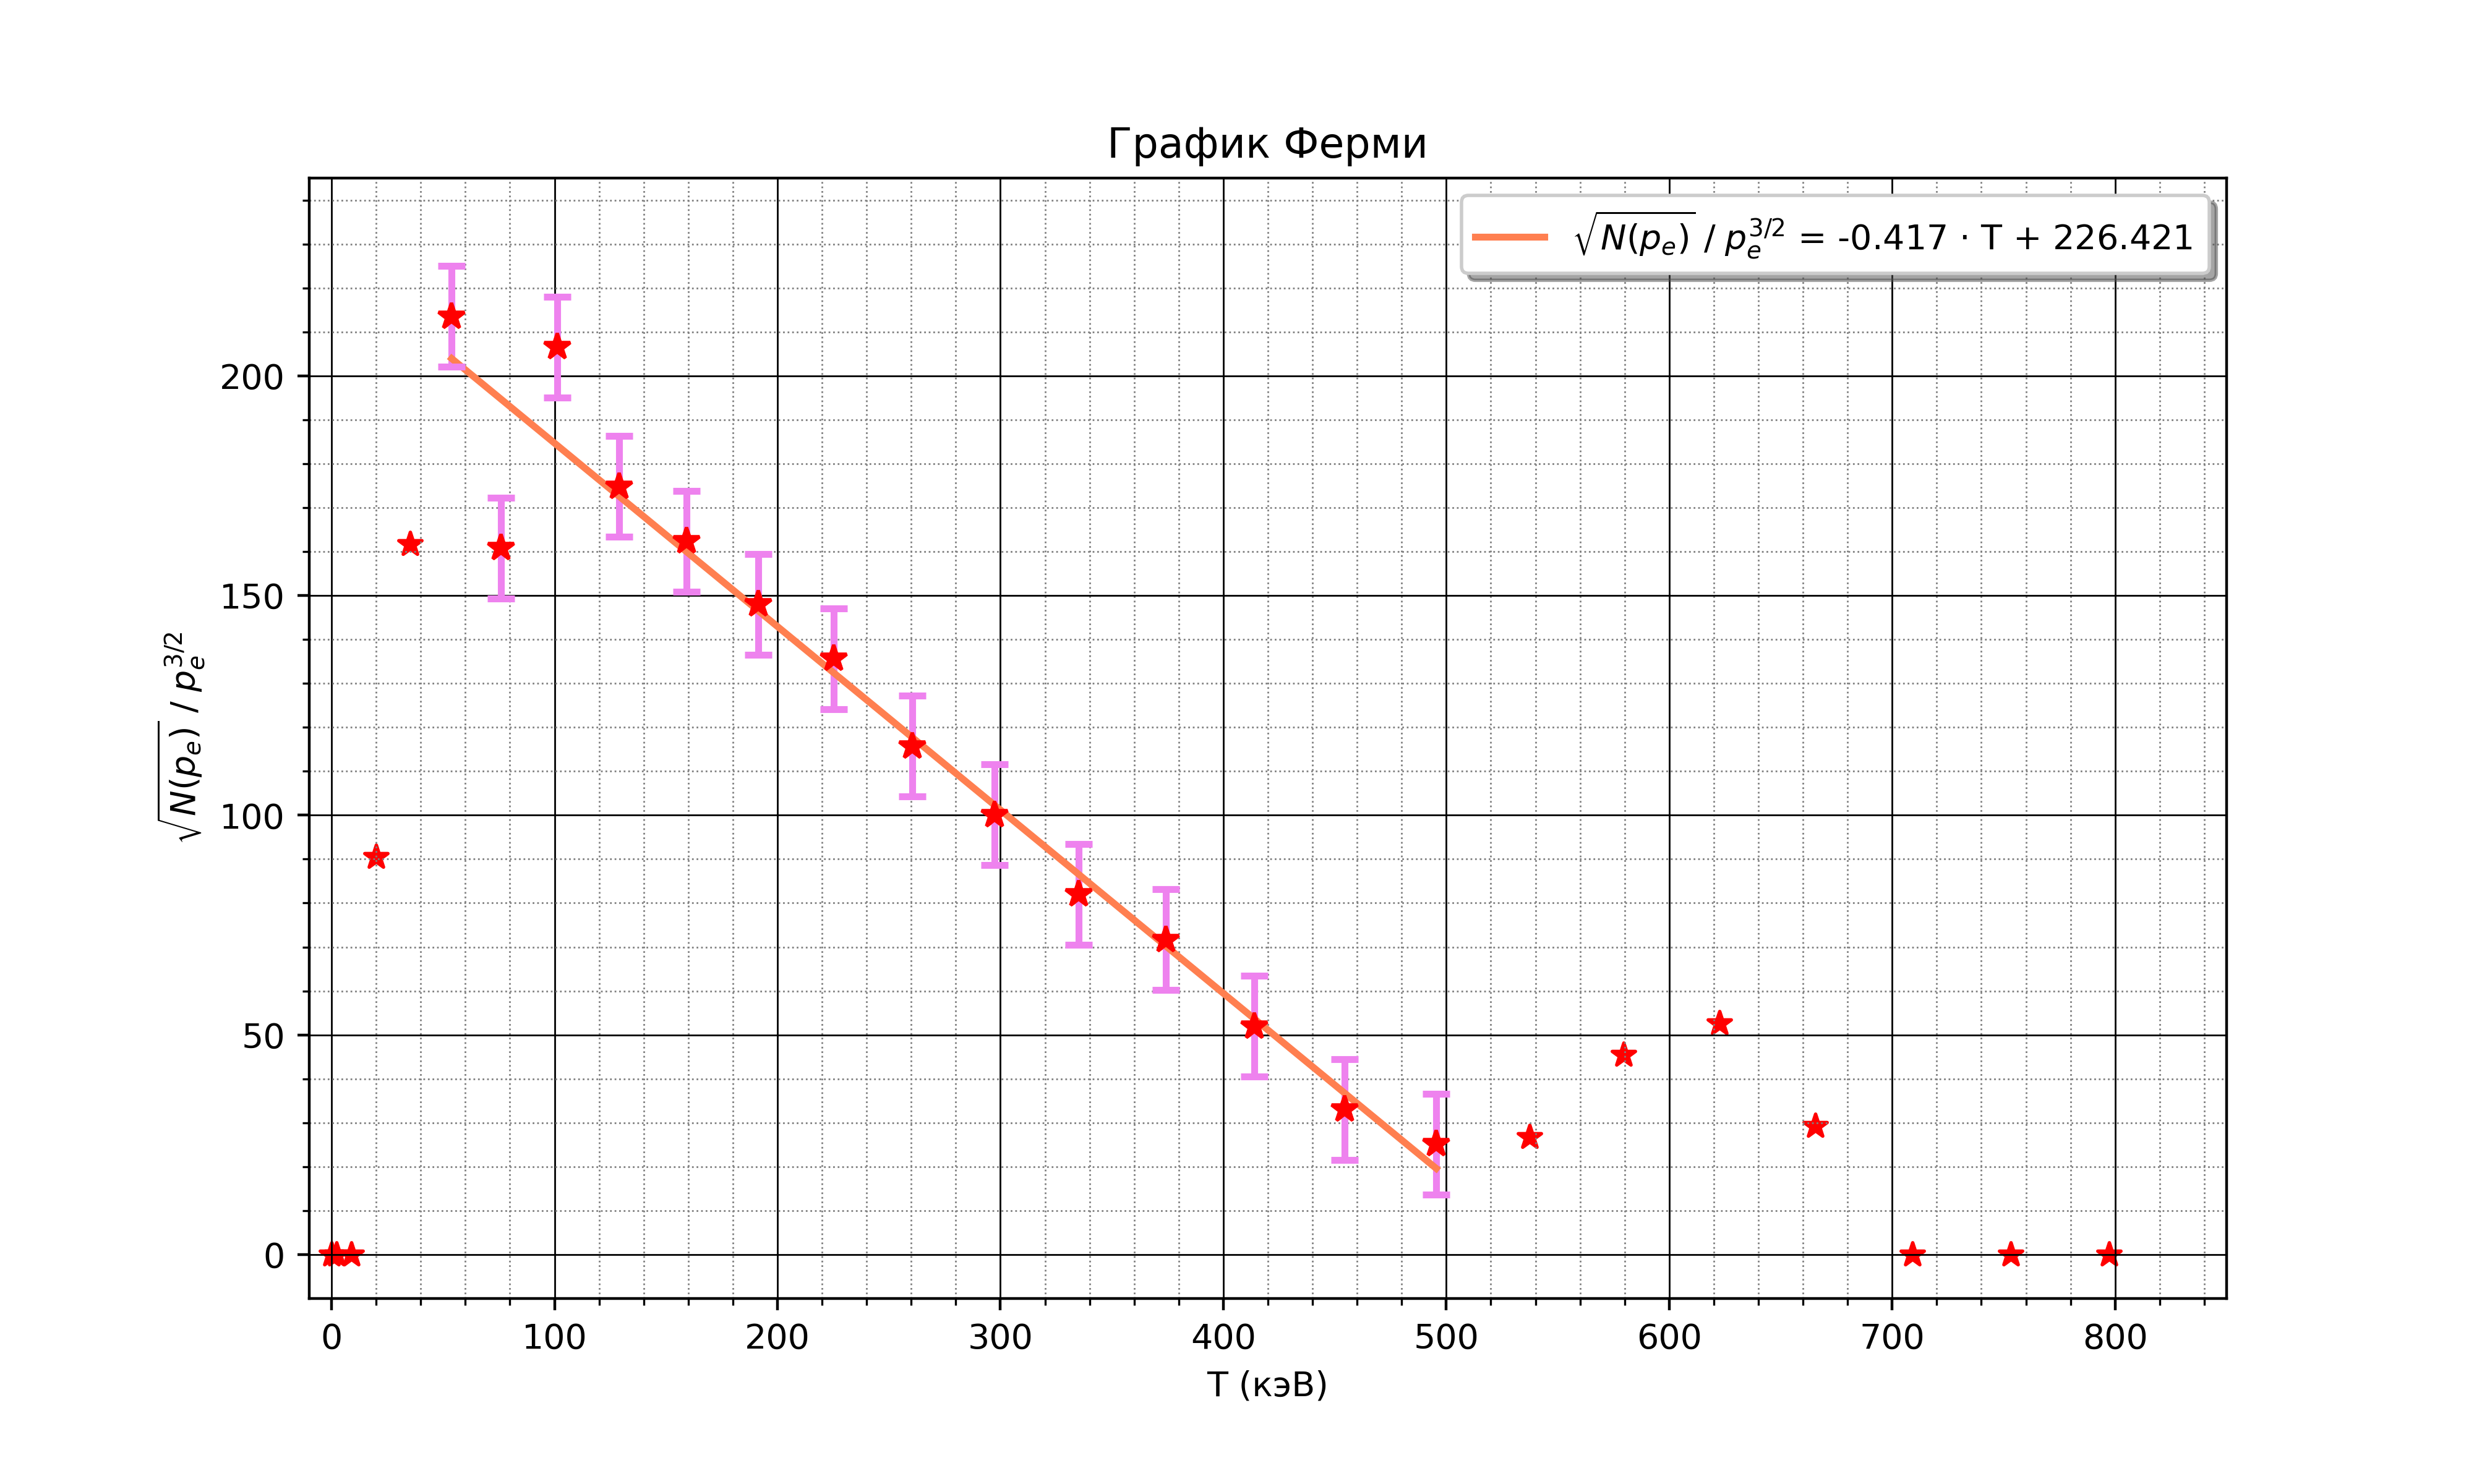
\includegraphics[scale = 0.7]{mkFermi.png}
        \caption{График Ферми}
        \label{g2}
        \end{center}
    \end{figure}

    По графику определим значение $T_{max} = 542.44 \pm 35.05\; \text{эВ} \;(6.46\%)$

\end{enumerate}

\section{Вывод}

В ходе работы было исследовано явление $\beta$-распада $^{137}Cs$. В спектр попали электроны, 
образованные в паре с антинейтрино при распаде, так же конверсионные электроны, испускаемые
возбужденными вторичными ядрами. С помощью графика Ферми $\sqrt{N(p_e)}\; / \; p^{3/2} \propto T_{max} - T$ 
было определено максимальное значение кинетической энергии $T_{max} = 542.44 \pm 35.05\; \text{эВ} \;(6.46\%)$.


\end{document}